\documentclass[a4paper,doc,11pt]{article}
%----------------------------------------------------------------------------------------
%	Paquetes y configuraciones
%----------------------------------------------------------------------------------------
\usepackage[numbers]{natbib}
\bibliographystyle{apalike}

\usepackage{amsfonts}
\usepackage{amsmath}
\usepackage{amssymb,amsthm}
\usepackage{enumerate}
\usepackage{enumitem}
\usepackage[utf8]{inputenc}
\usepackage[T1]{fontenc}
\usepackage{geometry}
\usepackage{hyperref}
\geometry{left=2cm,right=2cm,top=2.5cm,bottom=2.5cm}



\usepackage{url}
\def\UrlBreaks{\do\/\do-}
\usepackage{multirow}
\usepackage{multicol}
\usepackage{enumitem}
\usepackage{nicefrac}
\usepackage{graphicx}
\usepackage{stmaryrd}
\usepackage{dsfont}
\usepackage{bropd}
\usepackage{easybmat}
\usepackage{setspace}
\usepackage{comment}
\usepackage{mathpazo}
\usepackage{array}
\usepackage{commath}

\usepackage{sectsty}
\sectionfont{\centering\fontsize{13}{15}\selectfont}
\subsectionfont{\centering\fontsize{10}{10}\selectfont\scshape}

\newtheorem{theorem}{Theorem}[section]
\newtheorem{corollary}{Corollary}[theorem]
\newtheorem{proposition}{Proposition}[theorem]
\newtheorem{lemma}[theorem]{Lemma}
\newtheorem{definition}[theorem]{Definition}
\newtheorem{remark}[theorem]{Remark}
\newtheorem{example}[theorem]{Example}
\newtheorem{claim}{Claim}[subsection]




\usepackage[font=small]{caption}
\usepackage[font=small]{subcaption}
\captionsetup{subrefformat=parens}
\usepackage{booktabs} % nice headers for tables

\newcommand{\R}{\mathbb{R}}
\newcommand{\Z}{\mathbb{Z}}
\newcommand{\N}{\mathbb{N}}
\newcommand{\CC}{\mathcal{C}}
\newcommand{\llb}{\llbracket}
\newcommand{\rrb}{\rrbracket}

\DeclareMathOperator{\dom}{dom}
\DeclareMathOperator{\dist}{dist}
\DeclareMathOperator{\supp}{supp}
\setcounter{MaxMatrixCols}{20}


\SetLabelAlign{parright}{\parbox[t]{\labelwidth}{\raggedright#1}}
\allowdisplaybreaks


\usepackage[symbol]{footmisc}

\renewcommand{\thefootnote}{\fnsymbol{footnote}}


\linespread{1.38}

%---------------------------------------- Autoría ---------------------------------------- %
\usepackage{titling}
\predate{}
\postdate{\vspace{-2\baselineskip}}



\title{\bf
    \Large
    SMSTC 2021 
    \\
    Variational Methods of PDEs
}
\author{}%Andrés Miniguano Trujillo}
\date{}


\begin{document}
%\pagenumbering{Roman} 
\maketitle




%\newpage
%\tableofcontents


%%%%%%%%%%%%%%%%%%%%%%%%%%%%%%%%%%%%%%%%%%%%%%%%%%%
%\newpage
\section{User's Guide to Sobolev Spaces}
%\pagenumbering{arabic}

%%%%%%%%%%%%%%%%%
%%%%%%%%%%%%%%%%%
\subsection{Basic definitions}

Let \(\Omega \subset \R^N\) be an open set, \(N\) a positive integer, and \(p \in \R\) be such that \( 1\leq p \leq \infty\).

If we recall from Multi-variable Calculus, we know that if \(u\) is of class \( \CC^1(\Omega)\), then integration by parts yields
\[
    \int\limits_\Omega u \pd{\varphi}{x_i} \dif x = -\int\limits_\Omega \pd{u}{x_i} \varphi \dif x,
\]
whenever \( \varphi \equiv 0\) on \(\partial \Omega\). This gives us an alternative definition for the derivative of \(u\), which we can extend for measurable functions: Let \(u \in L^p(\Omega)\) and \(i \in \{1,\ldots,N\}\). If there exists \(g_i \in L^p (\Omega)\) such that
\begin{equation}
    \label{eq:1-pd}
    \int\limits_\Omega u \pd{\varphi}{x_i} \dif x = -\int\limits_\Omega g_i \varphi \dif x,
\end{equation}
for all \(\varphi \in \CC_c^{1} (\Omega)\)\footnote[2]{We denote \(\CC_c^{\infty} (\Omega)\) as the set of compactly supported functions of class \(\CC^1\) defined over \(\Omega\): 
\[
    \CC_c^{1} (\Omega) = \big\{ \varphi \in \CC^1(\Omega): \, \Omega \supset \supp \varphi = \{x: \varphi(x) \neq 0\} \text{ is compact } \big\}.
\]
}, then we say that \(g_i\) is the \emph{weak partial derivative of \(u\) with respect to \(x_i\)}, and for convenience we denote \( \pd{u}{x_i} := g_i \). Likewise, if there exist \( g_1, \ldots g_N \in L^p (\Omega)\) such that \eqref{eq:1-pd} is satisfied for all \( i \in \{1, \ldots, N\}\), then we say that the vector
\(
    \nabla u = 
    \begin{pmatrix}
        \pd{u}{x_1}, \ldots, \pd{u}{x_N}
    \end{pmatrix}
\)
is the \emph{weak derivative of \(u\)}.

The set of \(L^p (\Omega)\) functions that have weak derivatives form the \emph{Sobolev space} \( W^{1,p} (\Omega)\) defined by
\[
    W^{1,p} (\Omega) :=
    \left\{
        u \in L^p (\Omega): \,
        \begin{aligned}
        &\exists \{g_i\}_{i\in \{1,\ldots, N\}} \text{ such that } 
        \\
        &\int\limits_\Omega u \pd{\varphi}{x_i} \dif x = -\int\limits_\Omega g_i \varphi \dif x \quad \forall \varphi \in \CC_c^1 (\Omega) \quad \forall i \in \{1,\ldots,N\}
        \end{aligned}
    \right\}.
\]
This space is equipped with the norm\footnote{When there is no confusion, we will write \(W^{1,p}\) instead of \(W^{1,p} (\Omega)\).}
\[
    \|u\|_{W^{1,p}} :=  \|u\|_p + \sum_{i=1}^N \left\| \pd{u}{x_i} \right\|_p.
\]
We further note \(H^1(\Omega) := W^{1,2}(\Omega)\), which has the associated scalar product
\[
    (u,v)_{H^1} = (u,v)_{L^2} + \sum_{i=1}^N \left( \pd{u}{x_i} , \pd{v}{x_i} \right)_{L^2}.
\]
Notice that by the Cauchy–Bunyakovsky–Schwarz inequality the associated norm in  \(H^1\) is equivalent to the \(W^{1,2}\) norm.

\begin{proposition}
    The weak derivative is unique (almost everywhere).
\end{proposition}
\begin{proof}
    Let \(u \in W^{1,p}(\Omega)\), and suppose that there exists \(g_i\) and \( h_i\) such that both satisfy equation \eqref{eq:1-pd}, then
    \[
        0 = \int\limits_\Omega u \pd{\varphi}{x_i} \dif x - \int\limits_\Omega u \pd{\varphi}{x_i} \dif x = \int\limits_\Omega (g_i - h_i) \varphi \dif x
    \]
    for all \(\varphi \in \CC_c^1 (\Omega)\). By the Fundamental lemma of the calculus of variations, we have that \( g_i - h_i = 0\) almost everywhere, that is \( g_i = h_i\) (a.e).
\end{proof}

As weak derivatives are unique, there is no ambiguity in writing \(g_i = \pd{u}{x_i}\); i.e., our notation is consistent. Finally, we will see an important example of this theory, namely a function that is not globally \(\CC^1(\Omega)\) but has a weak derivative.

\begin{example}
    Let \(\Omega = (-1,1) \subset \R\) and consider the function \( u = |\cdot|\). Notice that \(u\) is not differentiable at \(0\); however we will determine its derivative. We have that integration by parts with any \(\varphi \in \CC_c^1 (\Omega)\) yields
    \begin{align*}
        \int\limits_\Omega u \varphi' \dif x
        =
        \int\limits_{0}^1 x \varphi'  \dif x
        -
        \int\limits_{-1}^0 x \varphi'  \dif x
        = 
        -\int\limits_{0}^1 \varphi  \dif x
        +
        \int\limits_{-1}^0 \varphi  \dif x
        =
        -\int\limits_\Omega g \varphi \dif x,
    \end{align*}
    where \(g\) is defined as
    \[
        g(x) = 
        \begin{cases}
            +1 & \text{if } x\in (0,1),
            \\
            -1 & \text{if } x\in (-1,0).
        \end{cases}
    \]
    Notice that by definition \(u\in L^p(\Omega)\) for every \(1 \leq p\leq \infty \), and it is clear that \(g \in L^p (\Omega)\) as well. 
    
    On the other hand, notice that \(g\) does \emph{not} belong to \( W^{1,p}(\Omega)\) for any \(1\leq p \leq \infty\). To see this, note that from Fundamental theorem of calculus and the fact that \(\varphi \in \CC_c^1 (\Omega)\):
    \[
        \int\limits_\Omega g \varphi' \dif x
        =
        \int\limits_0^1 \varphi' \dif x - \int\limits_{-1}^0 \varphi' \dif x
        =
        \varphi(1) - \varphi(0)  - \varphi(0) + \varphi(-1) = -2 \varphi(0).
    \]
    As a result, we would have that \( g = 2 \delta_0\), with \(\delta_0\) being Dirac's delta, which is a tempered distribution. On the other hand, from calculus we would need \(\od{g}{x} = 0\) for \( x\in (-1,0)\cup (0,1)\), which would imply that \( \varphi(0) = 0\) for all \(\varphi \in \CC_c^1 (\Omega)\), which is a contradiction.
\end{example}


%%%%%%%%%%%%%%%%%
%%%%%%%%%%%%%%%%%
\subsection{Approximation by smooth functions}

Let \(\Omega \subset \R^N\) be an open set, \(N\) a positive integer, \( 1\leq p < \infty\), and \( u \in L^p (\Omega)\). We would like see whether we can approximate \(u\) by a sequence of smooth functions.

From the previous subsection, we saw that \(\CC_c^1 (\Omega)\) is the space of \(\CC^1\) functions with compact support in \(\Omega\). Recall that the support of a function \(\varphi\) is a set \( K \subset \Omega\) such that is the smallest compact set where \( \varphi (x) = 0\) for \( x\in \Omega \setminus K\), and we note it \(\supp \varphi\). On a similar fashion, we denote \(\CC_c^k (\Omega)\) as the space of \(\CC^k\) functions with compact support in \(\Omega\), and likewise \(\CC_c^\infty(\Omega)\) as the space of \(\CC^\infty\) functions with compact support in \(\Omega\).

Note that a nonzero function \(\varphi \in \CC_c^\infty (\Omega)\) cannot be analytic, as its Taylor coefficients are zero for \( x \notin \supp \varphi\). An example of a nonzero function of this kind is 
\[
    e(x) := 
    \begin{cases}
        \lambda \exp \Big( \frac{1}{|x|^2-1} \Big) & \text{if } |x| < 1,
        \\
        0   & \text{if } |x| \geq 1,
    \end{cases}
\]
where \(\lambda\) is conveniently chosen such that \( \int e = \lambda \).
It can be shown that the \(n\)-th derivative of \(e\) is given by \( \od[n]{e}{x} = \frac{P_n(x)}{(x^2-1)^{2n}} e(x) \) for \( |x| < 1\), with \(P_n\) a polynomial \citep{Ball2019}; furthermore, \( e \in \CC_c^\infty (\R^N)\). 
It turns out that the function \(e\) defined above is part of a set of functions named \emph{mollifiers}. 

\begin{definition}
    A function \( \rho \in \CC_c^\infty(\R^N)\) is called a \emph{mollifier} if it is non-negative and 
    \(
        %\rho \geq 0,\qquad
        %\supp \rho \subset \overline{B(0,1)}, \qquad
        \int\limits_{\R^N} \rho(x) \dif x = 1.
    \)
\end{definition}

It is easy to generate a \emph{sequence of mollifiers} starting with a single function. For instance, if we consider the starndard mollifier \(e\) and let \(\varepsilon > 0\), then the functions
\[
    e_\varepsilon (x) := \varepsilon^{-N} e( \nicefrac x \varepsilon )
\]
determine a sequence of mollifiers as clearly they are non-negative and 
\[
    \int\limits_{\R^N} e_\varepsilon (x) \dif x = \int\limits_{\R^N} e(x) \dif x = 1.
\]
Moreover, \( \supp e_\varepsilon \subset B(0,\varepsilon) \). In Figure \ref{fig:1-Moll} we see the shape of the sequence \( e_\varepsilon\) for different values of \(\varepsilon\).
%

\begin{figure}
    \centering
    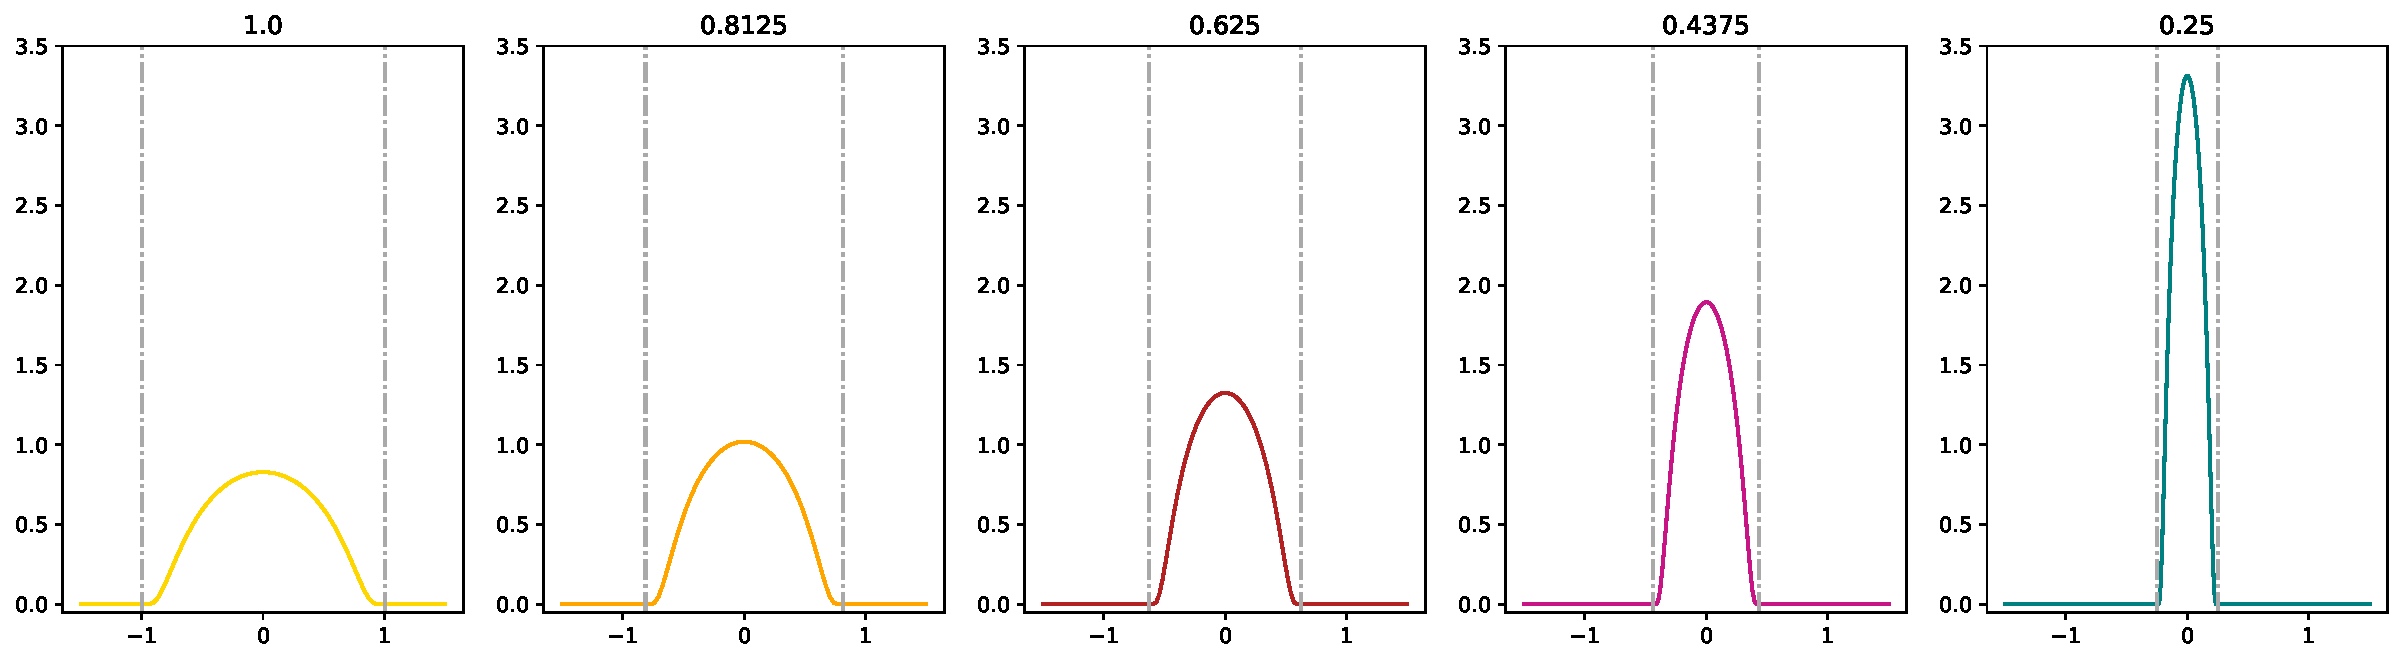
\includegraphics[width = \textwidth]{Fig-1_Moll.pdf}
    \caption{Mollifier sequence generated from the standard mollifier \(e\).\\ Each panel plots \(e_\varepsilon\) for a decreasing value of \(\varepsilon\). The vertical lines represent the cuts \( x = -\varepsilon\) and \(x = \varepsilon\). }
    \label{fig:1-Moll}
\end{figure}


%%%%%%%%%%%%%%%%%
%%%%%%%%%%%%%%%%%
\subsubsection{Convolution}

As we can see from Figure \ref{fig:1-Moll}, \( e_\varepsilon\) approximates Dirac's delta function, for small values of \(\varepsilon\). As a result, we can approximate \(u \in L^p (\Omega)\) by its \emph{mollification} given by
\[
    u_\varepsilon(x) := e_\varepsilon \star  u (x) = \int\limits_{\R^N} e_\varepsilon(x-y) u(y) \dif y.
\]
The mollification operation has the following properties:
\begin{lemma}
    Let \( 1\leq p < \infty\) and \( u \in L^p(\Omega)\). If we extende \(u \) to be zero outside \(\Omega\), then
    \begin{itemize}
        \item \(u_\varepsilon \in \CC_c^\infty (\R^N)\),
        \item \( \lim_{\varepsilon \to 0} \|u - u_\varepsilon\|_{L^p} = 0 \).
    \end{itemize}
    Moreover, if \(u \in W^{1,p} (\R^N)\), then \( \lim_{\varepsilon \to 0} \|u - u_\varepsilon\|_{W^{1,p}} = 0 \).
\end{lemma}

As we can expect, when \(\varepsilon \to 0\), we have that \( e_\varepsilon \) becomes \(\delta_0\) and we expect \( \delta_0 \star u_\varepsilon (x)  = u(x)\), for we have approximated \(L^p\) with smooth functions. In other words, the set \(\CC_c^\infty\) is dense in \(L^p (\Omega)\) for any \( 1 \leq p < \infty\). 

\begin{proposition}[Differentiation of product]
    Let \(u,v \in W^{1,p} (\Omega) \cap L^\infty (\Omega)\) with \( 1\leq p \leq \infty\). Then \(uv \in W^{1,p} (\Omega) \cap L^{\infty} (\Omega)\) and
    \[
        \pd{ }{x_i} (uv) = \pd{u}{x_i} v + u \pd{v}{x_i},
    \]
    for all \( i \in \{1,\ldots, N\}\).
\end{proposition}

We omit the proof of this proposition and refer the reader to Proposition 9.4 in \citep{Brezis2010}.

\begin{proposition}[Differentiation of composition]
    Let \(G \in \CC^1(\R)\) be such that \( G(0) = 0\) and \( |G'(x)| \leq M  \) for all \( x\in \R\) and for some constant \(M\). Let \( u\in W^{1,p} (\Omega)\) with \( 1\leq p \leq \infty\). Then \(G \circ u W^{1,p}(\Omega)\) and
    \[
        \pd{ }{x_i} (G \circ u) = (G'\circ u) \pd{u}{x_i}
    \]
    for all \( i \in \{1,\ldots, N\}\).
\end{proposition}

We omit the proof of this proposition and refer the reader to Proposition 9.5 in \citep{Brezis2010}.

\subsubsection{Higher order Sobolev Spaces}

All of the above discussion can be extended for higher order derivatives. For this end, it is convenient to have a compact notation for expressing mixed partial derivatives. A \emph{multi-index} \(\alpha\) is an \(N\)-tuple \( \alpha = (\alpha_1, \ldots, \alpha_N) \in \Z^N_+\), and we write \(|\alpha| = \alpha_1 + \ldots + \alpha_N\). 

Let \( \varphi \in \CC_c^\infty (\Omega)\). We define 
\[
    D^\alpha \varphi = \left( \pd[\alpha_1]{ }{x_1} \right) \cdots \left( \pd[\alpha_N]{ }{x_N} \right) u = \frac{\partial^{|\alpha|}}{ \partial x_1^{\alpha_1} \ldots \partial x_N^{\alpha_N} }.
\]
For example, if \(\beta = (2,0,1)\) and \(N = 3\), we get that \( |\beta| = 3\) and
\(
    D^\beta \varphi = \md{\varphi}{3}{x_1}{2}{x_3}{}.
\)

Using this notation, we can say that a function \( v \in L^{p}(\Omega)\) is the \( \alpha^\text{th}\) \emph{weak derivative} of a function \(u \in L^p(\Omega)\) if it satisfies
\[
    \int\limits_\Omega u D^\alpha \varphi \dif x = (-1)^{|\alpha|} \int\limits_\Omega v \varphi \dif x,
\]
for all \(\varphi \in \CC_c^{|\alpha|} (\Omega)\). As a result, we can now define the general Sobolev Spaces:

\begin{definition}
Let \(m\) be a non-negative integer and let \( 1\leq p \leq \infty\). The Sobolev Space \(W^{m,p} (\Omega)\) is the linear space of functions \( u \in L^p (\Omega)\) such that for each \(\alpha\), \(0 \leq |\alpha| \leq m\), the weak derivative \(D^\alpha\) exists and belongs to \(L^p (\Omega)\). Namely,
\[
    W^{m,p} (\Omega) :=
    \left\{
        u \in L^p (\Omega): \,
        \begin{aligned}
        &\forall \alpha \text{ with } |\alpha| \leq m, \exists g_{\alpha} \in L^p (\Omega) \text{ such that } 
        \\
        &\int\limits_\Omega u D^\alpha \varphi \dif x = (-1)^{|\alpha|}\int\limits_\Omega g_\alpha \varphi \dif x \quad \forall \varphi \in \CC_c^\infty (\Omega)
        \end{aligned}
    \right\}.
\]
\end{definition}

Just as with \(m = 1\), this space is also equipped with the norm
\[
    \|u\|_{W^{m,p}} :=  \sum_{0\leq |\alpha| \leq m} \| D^\alpha u \|_p,
\]
and it is a Banach space, see Theorem 8 \citep{Ball2019}. Moreover, the space \(W^{m,2}(\Omega)\) is often noted as \(H^m (\Omega)\) with the scalar product
\[
    (u,v)_{H^m} := \sum_{0\leq |\alpha| \leq m}  (D^\alpha u, D^\alpha v)_{L^2}.
\]
Notice that \(W^{0,p} (\Omega) = L^p (\Omega)\). Finally, the uniqueness of the derivative also follows from the Fundamental lemma of the calculus of variations, which we present now:

\begin{lemma}[Fundamental lemma of the calculus of variations]
    Let \( u \in L^1_{\mathrm{loc}} (\Omega)\) satisfy 
    \[
        \int\limits_\Omega u \varphi \dif x = 0
    \]
    for all \(\varphi \in \CC^k_c (\Omega)\), then \( u = 0 \) a.e. on \(\Omega\).
\end{lemma}
\begin{proof}
    Without loss of generality, we can consider the limit case \(k = \infty\). To see this, let \( g \in L^{\infty} (\R^N)\) be a function such that \( \supp g\) is compact and contained in \(\Omega\). We define \( g_\varepsilon = \rho_\varepsilon \star g\) with \(\rho_\varepsilon\) a mollifier. Let \(K\) be compact such that \( K \subset \Omega\). If \(\varepsilon < \dist (K,\partial \Omega)\), then for each \(x\) the function \( \rho_\varepsilon (x - y)\) belongs to \( \CC^\infty_c (\Omega) \).
    As a result
    \[
         \int\limits_\Omega u g_\varepsilon \dif x = 0
    \]
    for all \( x\in E\). However, we have that \( g_\varepsilon \to g\) in \(L^1 (\Omega)\), from where, via a subsequence, \( g_\varepsilon \to g\) almost everywhere on \(\R^N\). Moreover, as \( \|g_\varepsilon\|_\infty \leq \|g\|_\infty\), we can use Lebesgue's dominated convergence theorem to conclude \( \int\limits_\Omega u g\dif x = 0\). Now, we can pick \(g\) as the function
    \[
        g(x) = 
        \begin{cases}
            \mathrm{sign}(u) & \text{on } K,
            \\
            0   & \text{on } \R^N \setminus K.
        \end{cases}
    \]
    As a result, we have that \( \int\limits_K |u| \dif x = 0\) and thus \( u = 0\) a.e. on \(K\). Since this hold for any compact set \(K \subset \Omega\), we conclude that \( u = 0 \) a.e. on \(\Omega\). 
\end{proof}






%%%%%%%%%%%%%%%%%
%%%%%%%%%%%%%%%%%
\subsection{Extension operator}

It is often convenient to establish properties of functions in \(W^{1,p}(\Omega) \) starting with the case \( \Omega = \R^N\). As a result, it is useful to be able to extend a function \( u \in W^{1,p} (\Omega)\) to a function in \( W^{1,p} (\R^N)\). 

We start with some notation. Given \( x \in \R^N\), we will write
\[
    x = (x', x_N) \text{ with } x' \in \R^{N-1}, \qquad 
    x' = (x_1, \ldots, x_{N-1}).
\]
Moreover, we will notate \(\R^N_+\) as the set
\[
    \R^N_+ := \{ x = (x',x_N): \, x_N > 0 \}.
\]

\begin{lemma}
    Given \( u \in W^{1,p} (\R^N_+)\) with \( 1 \leq p \leq \infty\), one defines the function \(u^*\) on \(\R^N\) to be the \emph{extension by reflection}, that is,
    \[
        u^* (x',x_N) = 
        \begin{cases}
            u (x',x_N) & \text{if } x_N > 0,
            \\
            u (x',-x_N) & \text{if } x_N < 0.
        \end{cases}
    \]
    Then \( u^* \in W^{1,p} (\R^N)\) and
    \[
        \|u^*\|_{L^p (\R^N)} \leq 2 \|u\|_{L^p (\R^N_+)},
        \qquad
        \|u^*\|_{W^{1,p} (\R^N)} \leq 2 \|u\|_{W^{1,p} (\R^N_+)}.
    \]
    In fact, this comes from
    \[
        \pd{u^*}{x_i} = \left( \pd{u}{x_i} \right)^* 
    \]
    for \( i \in \{1,\ldots, N-1\}\) and
    \[
        \pd{u^*}{x_N} = \left( \pd{u}{x_i} \right)^{\square}
        =
        \begin{cases}
            \pd{u}{x_N} (x',x_N) & \text{if } x_N > 0,
            \\
            -\pd{u}{x_N} (x',-x_N) & \text{if } x_N < 0.
        \end{cases}
    \]
\end{lemma}
\begin{proof}
    Let \(\eta \in \CC^\infty\) be such that 
    \[
        \eta (t) =
        \begin{cases}
            0   &\text{if } t < \nicefrac 1 2
            \\
            1   & \text{if } t > 1. 
        \end{cases}
    \]

    We shall use a sequence \((\eta_k)_{k\in \N^*}\) of functions in \(\CC^\infty (\R)\) defined by
    \[
        \eta_k (t) = \eta (kt)
        =
        \begin{cases}
            0   &\text{if } t < \nicefrac{1}{2k}
            \\
            1   & \text{if } t > \nicefrac{1}{k}. 
        \end{cases}
    \]
    
    \begin{figure}
    \centering
    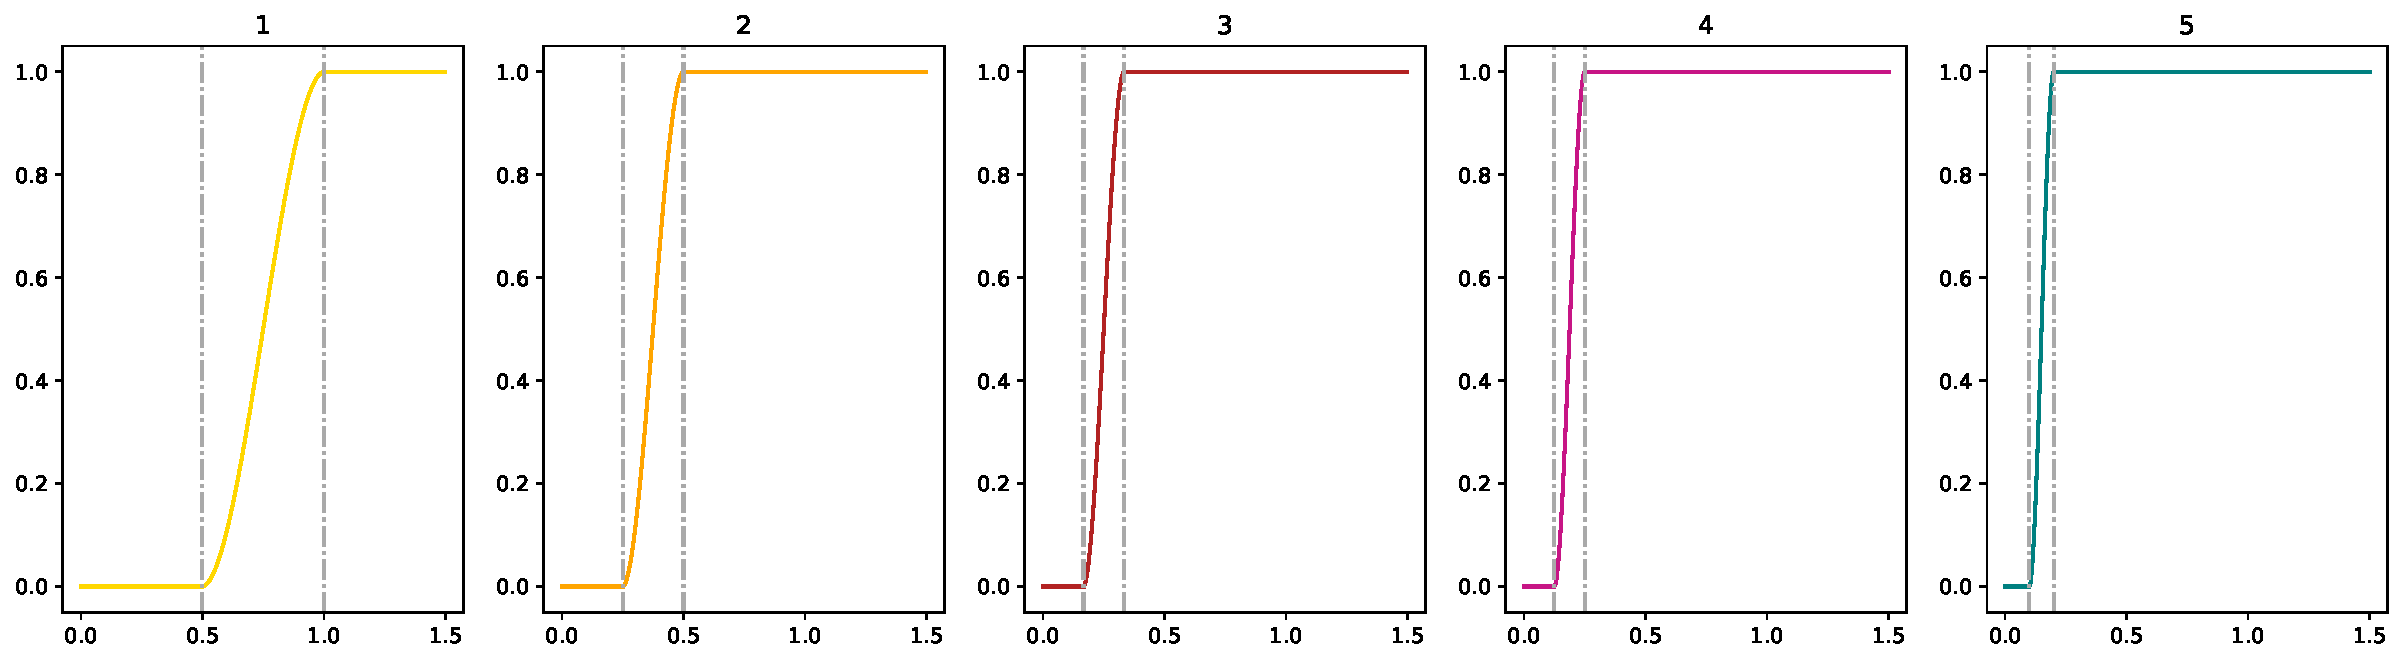
\includegraphics[width = \textwidth]{Fig-2_Ext.pdf}
    \caption{A representation of \(\eta\) and the sequence \(\eta_k\) for the first values of \(k \in \N^*\).\\ The vertical lines correspond to \( x = \nicefrac 1 k\) and \(x = \nicefrac{1}{2k}\). }
    \label{fig:2-Ext}
\end{figure}
    
    Let \(\varphi \in \CC^1_c (\R^N)\) and \( 1 \leq i \leq N-1\). By definition we have that
    \[
        \int\limits_{\R^N} u^* \pd{\varphi}{x_i} \dif x = 
        \int\limits_{\R^N_+} u \pd{\varphi}{x_i} \dif x 
        +
        \int\limits_{\R^N_-} u(x',-x_N) \pd{\varphi}{x_i} \dif x 
        =
        \int\limits_{\R^N_+} u \pd{\psi}{x_i} \dif x ,
    \]
    where \(\phi(x', x_N) := \varphi(x', x_N) + \varphi(x', -x_N)\). The function \(\psi\) does not in general belong to \( \CC_c^1 (\R^N)_+\), and thus it cannot be used as a test function in the definition of \( W^{1,p} \). On the other hand, we note that \( \eta_k (x_N) \psi (x', x_N) \in C_c^1 (\R^N_+)\) and thus
    \[
        \int\limits_{\R^N_+} u \pd{ }{x_i} (\eta_k \psi) \dif x 
        =
        -\int\limits_{\R^N_+} \pd{u}{x_i} \eta_k \psi \dif x.
    \]
    Since \( \pd{ }{x_i} (\eta_k \psi) = \eta_k \pd{\psi}{x_i} \), we have
    \[
        \int\limits_{\R^N_+} u \eta_k \pd{ }{x_i} \psi \dif x 
        =
        -\int\limits_{\R^N_+} \pd{u}{x_i} \eta_k \psi \dif x.
    \]
    Passing to the limit as \(k \to \infty\) (by Lebesgue's dominated convergence theorem), we obtain
    \[
        \int\limits_{\R^N_+} u \pd{ }{x_i} \psi \dif x 
        =
        -\int\limits_{\R^N_+} \pd{u}{x_i} \psi \dif x.
    \]
    As a result, we have gotten
    \[
        \int\limits_{\R^N} u^* \pd{\varphi}{x_i} \dif x = 
        -\int\limits_{\R^N_+} \pd{u}{x_i} \psi \dif x =
        -\int\limits_{\R^N} \left(\pd{u}{x_i} \right)^* \psi \dif x.
    \]
    
    
    Now, for the case \( i = N\), we have
    \[
        \int\limits_{\R^N} u^* \pd{\varphi}{x_N} \dif x = 
        \int\limits_{\R^N_+} u \pd{\chi}{x_N} \dif x ,
    \]
    where \(\chi(x', x_N) := \varphi(x', x_N) - \varphi(x', -x_N)\). Note that \( \chi(x',0) = 0\), and thus there exist a constant \(M\) such that \(|\chi(x',x_N)| \leq M|x_N|\) on \(\R^N\). Since \( \eta_k \chi \in C_c^1 (\R^N_+)\), we have
    \[
        \int\limits_{\R^N_+} u \pd{ }{x_N} (\eta_k \chi) \dif x 
        =
        -\int\limits_{\R^N_+} \pd{u}{x_N} \eta_k \chi \dif x.
    \]
    But \( \pd{ }{x_N} (\eta_k \chi) = \eta_k \pd{\chi}{x_N} + k \eta'(k x_N) \chi \). Notwithstanding, we further have
    \[
        \left| \int\limits_{\R^N_+} u k \eta'(k x_N) \chi \dif x \right|
        \leq k M C \int\limits_{\R^N_+ \cap \{|x_N| < \nicefrac 1 k\}} |u| x_N \dif x
        \leq MC \int\limits_{\R^N_+ \cap \{|x_N| < \nicefrac 1 k\}} |u| \dif x,
    \]
    thus
    \[
        \int\limits_{\R^N_+} u k \eta'(k x_N) \chi \dif x \to 0 
    \]
    as \(k \to \infty\). As a result, we have that
    \[
        \int\limits_{\R^N_+} u \pd{ }{x_N} (\chi) \dif x 
        =
        -\int\limits_{\R^N_+} \pd{u}{x_N} \psi \dif x.
    \]
    Finally, we have 
    \[
        \int\limits_{\R^N_+} \pd{u}{x_N} \chi \dif x 
        =
        \int\limits_{\R^N} \left( \pd{u}{x_N} \right)^\square \varphi \dif x.
        \qedhere
    \]
\end{proof}

It is worth mentioning that this construct can be carried out for \(W^{1,p}(\Omega)\), when \(\Omega\) is a \(\CC^1\) domain, see Theorem 9.7 in \citep{Brezis2010}.

%%%%%%%%%%%%%%%%%
%%%%%%%%%%%%%%%%%
\subsection{Sobolev Inequalities}

The Sobolev Inequalities, also known as Sobolev embeding theorems, are a group of results that allow to recover some regularity from \(W^{1,p}\) spaces. 

\begin{theorem}
    Let \( \Omega \subseteq \R^N \)  be \( \R^N\), open of class \(\CC^1\) with \(\partial \Omega\) bounded, or \( \R^N_+\). For \( 1\leq p \leq \infty\), we have
    \begin{align}
        W^{1,p} (\Omega) \subset L^{p^*} (\Omega) && \text{where } \quad\frac{1}{p^*} = \frac{1}{p} - \frac{1}{N} && \text{if } p < N,
        \\
        W^{1,p} (\Omega) \subset L^{q} (\Omega) && \text{for all } \quad q \in [p,+\infty) && \text{if } p = N,
        \\
        W^{1,p} (\Omega) \subset L^{\infty} (\Omega) &&  && \text{if } p > N;
    \end{align}
    and all the injections are continuous. Moreover, if \(p > N\) we have, for all \(u \in W^{1,p} (\Omega)\),
    \[
        |u(x) - u(y)| \leq C\|u\|_{W^{1,p}} |x-y|^\alpha \qquad \text{a.e. }  x,y \in \Omega,
    \]
    with \(\alpha = 1 - \nicefrac N p\) and \(C\) depends only on \(\Omega\), \(p\), and \(N\). In particular, \( W^{1,p} (\Omega) \subset C(\bar \Omega)\).
\end{theorem}















\vspace{2\baselineskip}

Example cite:
\citet{Brezis2010}, \citep{Brezis2010}





%%%%%%%%%%%%%%%%%%%%%%%%%%%%%%%%%%%%%%%%%


\section*{Availability of data, material, and code}
{
%\small

All the files and this document are available as in the following repository:
\begin{quote}
    \noindent \href{https://github.com/andresrmt/Variational-Methods-for-PDEs}{\texttt{https://github.com/andresrmt/Variational-Methods-for-PDEs}}
\end{quote}



}

%%%%%%%%%%%%%%%%%%%%%%%%%%%%%%%%%%%%%%%%%
%%%%%%%%%%%%%%%%%%%%%%%%%%%%%%%%%%%%%%%%%
\newpage


\bibliography{Cites}

\end{document}



